
\section{Introduction}

The demands of everyday life require us to flexibly shift our attention between many different aspects of the visual world. When researchers operationalize such behaviors they often task observers to select information either from a specific location or with a particular feature. The difference between covert spatial attention and feature-based attention seems intuitive at first glance and may reflect a real physiological difference in how selection is implemented by the brain. It is also possible that space is not privileged over other features in visual cortex, and that instead, selection of information is a generic computation.

There is some evidence that selection by location and feature differ in subtle ways. One large difference is that feature-based attention operates as a global (spatially non-specific) form of selection, e.g. for motion direction and color \citep{Saenz2002-fs}. Another difference is that selection by location may operate at a slightly faster rate than selection by feature \citep{Liu2007-ed,Hillyard1984-qk,Harter1982-vj}. Spatial selection is also primary in some ways \citep{Soto2004-cs,Tsal1988-qx}. This has been demonstrated by showing that subjects are more likely to recall letters near an attended location over letters of a similar color at distant locations \citep{Tsal1988-qx} as well as by showing that errors in letter recall occur for spatial neighbors but not for color-matched distant neighbors \citep{Snyder1972-og}. It has also been proposed that to create objects out of visual properties they must be bound together by location \citep{Treisman1980-gu}, making location primary over other features. Other comparisons have suggested that spatial and featural selection are impacted by perceptual noise in different ways \citep{Ling2009-rq}. All of these results indicate that under the right conditions small differences exist between these two basic forms of selection.

Are the small differences between spatial and feature-based selection a result of a difference in how selection is implemented in the brain? We sought to answer this question by building a stimulus in which selection by location, color, and motion direction could be compared on a shared perceptual metric. We used this stimulus in two tasks, a perceptual averaging task and a working memory estimation task. In both tasks observers were asked to select information either by spatial location or according to a stimulus property (either motion direction or color) while reporting about a third property. In both data sets we show that sensitivity is extremely similar between each form of selection and that any differences in performance are accounted for by changes in bias to the irrelevant dot patches. Finally, we suggest possible implementations by which a common computation could select sensory representations and account for the behavioral observations.

\section{Methods}

\subsection{Observers}
In total 13 observers were subjects for the experiments (x female, y male, mean age z, age range a - b). All observers except one (who was an author) were naive to the intent of the experiments. One observer was excluded during the initial training sessions due to an inability to maintain appropriate fixation (see eye-tracking below). Procedures were approved in advance by the Stanford Institutional Review Board on human participants research and all observers gave prior written informed consent before they participated in the experiment. When necessary, observers wore corrective lenses to correct their vision to normal. Observers were filtered prior to inclusion based on self-reported color vision and tested for colour vision deficits using the Ishihara test \citep{Ishihara1987-wo}, one observer had to be excluded based on the test results.

Seven of the observers completed the averaging task, completing on average 988 trials (range 280 - 1475) over a series of ninety minute session. Five of the observers completed the estimation task, completing on average 2290 trials (range 1770 - 2613) over a series of sixty minute sessions. 

\subsection{Hardware setup for stimulus and task control}

Visual stimuli were generated using MATLAB (The Mathworks, Inc.) and MGL \citep{Gardner2018-uq}. Stimuli were displayed on a 22.5 inch VIEWPixx LCD display (resolution of 1900x1200, refresh-rate of 120 Hz) and responses collected via keyboard. Output luminance and spectral luminance distributions were measured for the LCD display with a PR650 spectrometer (Photo Research, Inc.). The gamma table for each display was dynamically adjusted at the beginning of each trial to linearize the luminance display such that the full resolution of the 8-bit table could be used to display the maximum contrast needed. The luminance spectra were used to compute a transformation matrix from the CIELAB color space to the RGB output of the screen, such that the a* and b* dimensions could be separately manipulated without changing the luminance (L*). Other sources of light were minimized during behavior. Observers used a circular volume controller to submit their responses in angle space (Powermate USB, Griffin Audio).

\subsection{Eye tracking}

Eye-tracking was performed using an infrared video-based eye-tracker at 500 Hz (Eyelink 1000; SR Research). Calibration was performed throughout each session to maintain a validation accuracy of less than 1 degree average offset from expected using a thirteen-point calibration procedure. Trials were initiated by fixating the central cross for 300 ms and canceled on-line when an observer’s eye position moved more than 1.5 degree away from the center of the fixation cross for more than 300 ms. During training and before data collection observers were excluded from further participation if we were unable to calibrate the eye tracker to an error of less than 1 degree of visual angle or if their canceled trial rate did not drop to near zero.

\subsection{Experimental design}

\subsubsection{Averaging task}

Stimuli consisted of two pairs of dot patches, to the left and right of a central fixation cross (0.5 x 0.5 deg). The dot patches were circular regions centered 8 degrees eccentric with a diameter of 10 deg, covering from 3 to 13 deg along the horizontal axis and -5 to +5 deg along the vertical axis. Each side had two dot patches was filled with moving dots (0.2 dots / deg$^2$, per set, 0.3 deg diameter). Dots within a patch were given an identical color and moved in the same direction at 3.5 deg / s. Dots were `alive' for 0.25 s before vanishing and reappearing immediately at a new random location. One patch on each side was colored yellow and one blue (90 deg and 270 deg, in a* b* space). 

On each trial in the averaging task observers were asked to report the average motion direction of two dot patches (Fig. \ref{fig:c4f1}. Before each set of 20 trials observers were told how they would select the two dot patches with the phrase ``cue side'' or ``cue color'' shown at fixation. Each trial was initiated by the observer fixating the central cross for 0.5 s. This was followed by a 0.75 s cue, either a line to the left or right or a miniature patch of colored dots. The feature instructed the observers about which two dot patches they would need to average: either the two on the left, on the right, or the two yellow or blue patches (one on the left and one on the right). A 0.75 s delay followed. During the stimulus period the dot patches began moving coherently in random directions. The target patches were constrained to be less than 135 degrees apart, to avoid confusion about the correct response (when 180 degrees apart, two possible answers are correct). Observers were shown the stimulus for a variable duration of 0.25 to 0.75 s, then allowed unlimited time to rotate the response wheel and make a response. Feedback was given by showing the actual average motion direction (see Figure). Each trial was followed by a brief inter-trial interval (0 - 2 s, uniformly distributed).

\subsubsection{Psychophysical distance}

We report all of our results according to the normalized psychophysical distance between angles in motion direction and color space, rather than the physical units. This is based on a recent result showing that in working memory estimation tasks, correctly taking into account the psychophysical distance is critical to correctly interpreting data \citep{Schurgin2018-vi}. In brief, the motivation for this scaling is that beyond a certain degree distance the ``psychophysical'' distance becomes compressed. The intuition here is that if you are trying to compare N or NE to E, it's easy to tell that NE and E are closer. But if you are trying to quickly compare N or NE to S, the task becomes more difficult and there is little difference between that comparison and N and NE to SW. The re-scaling sets the `distance' between two angles to the normalized sensitivity according to the task described above. Without this re-scaling of distances it's easy to mistake poor sensitivity for a high lapse rate. The authors of \citet{Schurgin2018-vi} as well as others \citep{Bays2014-ym} convincingly demonstrate that in fact lapse rates are consistently low in difficult working memory tasks. When observers appear to be guessing they are actually making low-probability choices with high-confidence. For our purposes we approximated the psychophysical scaling by fitting a sigmoidal function to data available in that paper: 

\begin{equation}
    d(x) = 1.1\frac{x^{1.5}}{x^{1.5}+35^{1.5}}
    \label{eqn:c5psycho}
\end{equation}

This equation therefore transforms the distance $x$ between two motion directions or colors (in a* b* angle space) to the normalized psychophysical distance $d$. Unlike degree distance, the normalized psychophysical is set up such that an observer perceives the difference between 0 and 0.5 (0 and 31 deg, respectively) as equal to the difference between 0.5 and 1 (31 and 180 deg).

\subsubsection{Estimation task}

On each trial in the estimation task observers were asked to report about either the color or motion direction of a single dot patch. Before each block of 40 trials observers were told which feature would be reported with either the phrase ``report color'' or ``report direction'' appearing on the screen. Key to the task was that although observers ultimately reported about only one dot patch they could be cued to remember just that patch, or multiple patches, during a brief delay period. Each trial consisted of the following sequence (Fig. \ref{fig:c4f4}): a fixation period (0.5 s), a pre-cue indicating which patches needed to be memorized (0.75 s), an inter-stimulus interval (0.75 s), stimulus presentation (0.25 s), a delay (1 s), a post-cue resolving which dot patch should be reported (0.75 s) and then unlimited time to report a response. The inter-trial interval was 0 - 2 s, sampled randomly from a uniform distribution. The stimulus duration (0.25 s) was chosen based on the averaging task to ensure that the task was difficult for participants but not impossible. 

\subsubsection{Estimation task data analysis}

To analyze the results of the estimation task we fit a modified version of the ``target confusability competition'' model from \citet{Schurgin2018-vi}. The model is based on the idea that noisy internal channels are independently competing to represent a stimulus (Fig. \ref{fig:c4f4}a). On each trial the model proceeds in two steps. First, the stimulus (or stimuli) are encoded by the channels, setting their mean response. The tuning profile of each channel comes from the normalized psychophysical distance (Eq. \ref{eqn:c5psycho}). As an example, the encoding step the response of a small set of channels (Fig. \ref{fig:c4f4}a) to a stimulus with an angle of zero is shown (Fig. \ref{fig:c4f4}b). Each channels response is distributed as follows:

\begin{equation}
    C_{\theta}(x) = \mathcal{N}(\mu = \alpha d(x-\theta),\sigma=1)
    \label{eqn:c5channel}
\end{equation}

Where $\theta$ is the preferred orientation for that channel and $d$ is Eq. \ref{eqn:c5psycho}. $\alpha$ is an amplitude parameter which controls the scaling of the response and is the only free parameter in the model.

Once a stimulus is encoded by a set of responses the second step in the model is to find the observer's behavioral response by taking the maximum response over the channels. Because each channel has independent normally-distributed noise, the likelihood of each channel winning can be computed as the conditional probability of the channel exceeding all of the other channels. We approximate this likelihood by numerically integrating the likelihood over channel responses, as follows:

\begin{equation}
    \matchcal{L}(\theta) = \int_{0}^{\infty} P(x_{\theta}=a) \prod_{j\neq \theta}P(x_j < a) \mathrm{d}a
    \label{eqn:c5like}
\end{equation}

Where $P(x)$ is normally distributed, according to (Eq. \ref{eqn:c5channel}). To compute the full likelihood distribution we evaluate Eq. \ref{eqn:c5like} at all values of $\theta$.

Because the response calculation is analogous to signal detection the $\alpha$ parameter in Eq. \ref{eqn:c5channel} is actually the sensitivity of the channel (i.e. $d'$). We fit this free parameter to the responses of each observer by maximizing the likelihood of the observed data using Bayesian adaptive direct search \citep{Acerbi2017-xz} in MATLAB.

We performed the model fitting step in such a way as to separate an observer's bias (i.e. likelihood of responding about the incorrect dot patch) from their sensitivity (i.e. their variability in response quality, for a given dot patch). We modeled the observer's trial-by-trial response as a combination of a likelihood function for each stimulus patch (Eq. \ref{eqn:c5like}) with a set of bias parameters.

\begin{equation}
    \matchcal{L}(\theta) = \beta_{target}\matchcal{L}_{target} + \beta_{side}\matchcal{L}_{side} +\beta_{feature}\matchcal{L}_{feature} +\beta_{distractor}\matchcal{L}_{distractor}
\end{equation}

Where the terms \textit{target}, \textit{side}, \textit{feature}, and \textit{distractor} correspond to the dot patch that was reported on the trial, the patch on the same side, the patch on the opposite-side with matched-feature, and the patch on the opposite-side with mismatched-feature, respectively (Fig. \ref{fig:c4f5}). The actual $\beta$ values were constrained so that $\beta_{target}+\beta_{side}+\beta_{feature}+\beta_{distractor}=1$, by calculating them from three intermediate values:

\begin{equation}
    \beta_{target} = \beta_{s} * \beta_{f}
\end{equation}

\begin{equation}
    \beta_{side} = \beta_{s} * (1-\beta_{f})
\end{equation}

\begin{equation}
    \beta_{feature} = (1-\beta_{s}) * (1-\beta_{d})
\end{equation}

\begin{equation}
    \beta_{distractor} = (1-\beta_{s}) * \beta_{d}
\end{equation}

Where $\beta_s$, $\beta_f$, and $\beta_d$ are each constrained to the range [0,1]. Setting $\beta_s=1$ and $\beta_f=1$ means that the observer is always choosing the target and never incorrectly being biased to respond about the other three dot patches (i.e. $\beta_{target}=1$).

In sum, we fit four sensitivity parameters ($\alpha$) and three bias parameters ($\beta$) for the data set in which observers selected by location or color (and reported motion direction) and separately for the data set in which they selected by location or motion direction (and reported color).

\subsection{Implementing attention in a channel linking model}

The channels in the behavioral model described above have tuning which, by definition, matches the behavior. In reality, the psychophysical scaling is a result of the readout process from neurons tuned with much sharper functions \citep{Bays2014-ym,Bays2019-ni}. To explore how attention might change the responses of neurons we explored how to connect sharp tuning functions, such as those neurons might have, to the psychophysical space described above.

In this simulation we assumed that channels had a Von Mises tuning with a relatively sharp profile (Fig. \ref{fig:c4f7}a). As before the response of each channel had independent Gaussian noise at the time of stimulus encoding. To read out from these channels we computed:

\begin{equation}
    \hat{\theta} = \mathrm{arg}\,\mathrm{max}_{\theta} \sum_{i} r_i \overline{r}_i (\theta)
    \label{eqn:c5readout}
\end{equation}

Where $r$ is the response of each channel to the stimulus and $\overline{r}$ is the response of that channel in the absence of noise. 

To simulate different models of attention we either applied a gain to the noisy channel responses or changed the set of mean channel tuning values. When `shifting' the tuning it is necessary to also shift the expected readout. 

\section{Results}

\begin{figure}
\centering
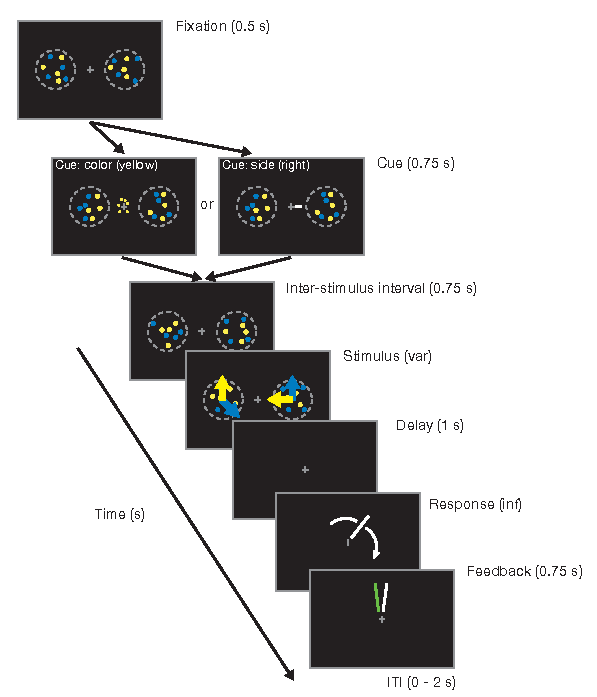
\includegraphics[keepaspectratio,width=0.50\textwidth]{figs_c4/f1_task.pdf}
\caption[Averaging task]{Motion direction averaging task. Observers were asked to select two out of four random dot patches and average their motion direction. Observers initiated trials by fixating a central cross, causing the two dot patches to appear with incoherent motion. A cue indicated whether they should select the left or right patches (spatial selection) or the yellow or blue ones (feature-based selection). After a brief delay the dot patches each began moving in random directions, before vanishing again for a second short delay. Finally, observers used a rotating wheel to report the \textit{average} direction of motion for the two dot patches they were asked to select. Feedback was given by indicating the true average motion direction.}
\label{fig:c4f1}
\end{figure}

We characterized human perceptual sensitivity to the average motion direction of two dot patches, while asking observers to select the two patches either based on their common location or a shared feature (Fig. \ref{fig:c4f1}. To measure perceptual sensitivity we recorded each observer's estimation error relative to the true average motion direction. We found that whether observers selected the two dot patches by spatial location (left or right) or by feature (yellow or blue), their estimation errors remained nearly identical (Fig. \ref{fig:c4f2}). Consistent with the task design we found that giving observers a longer stimulus (Fig. \ref{fig:c4f3}a) or a smaller angle difference between the two dot patches (Fig. \ref{fig:c4f3}b) improved sensitivity slightly. 

\begin{figure}
\centering
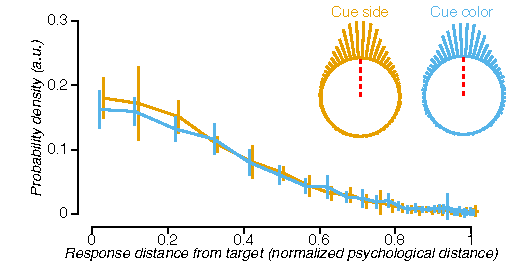
\includegraphics[keepaspectratio,width=0.5\textwidth]{figs_c4/f2_aca_perf.pdf}
\caption[Estimation error during averaging]{Estimation error during the averaging task. A histogram displaying the average proportion of responses at each distance from the true average motion direction (0) is shown, averaged across observers. Selection by spatial location (i.e. averaging the two patches on the right or left) is shown in yellow, and selection by color (i.e. averaging the two yellow or blue patches) is shown in blue. The two inset plots show the same histogram but in a circular space, with a red dashed line indicating the true average. Note that the x-axis has been re-scaled from degrees to psychophysical distance, see Methods for details.}
\label{fig:c4f2}
\end{figure}

\begin{figure}
\centering
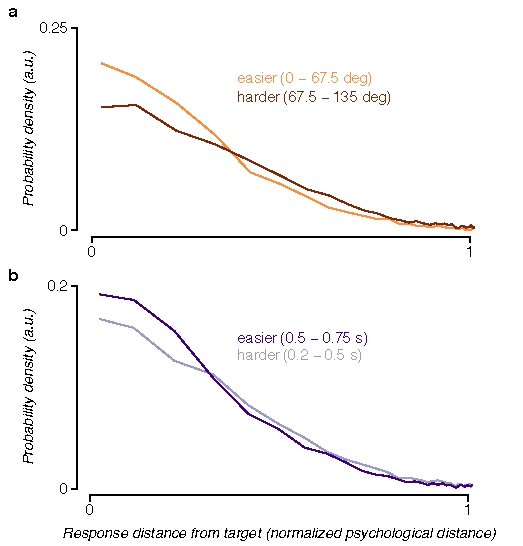
\includegraphics[keepaspectratio,width=0.45\textwidth]{figs_c4/f2_aca_parameters.pdf}
\caption[Parameters that control difficulty of averaging]{Averaging difficulty is controlled by stimulus duration and angle distance between patches. (a) The average estimation error across observers is shown for a median split of the angle difference between the two dot patches that were averaged. (b) As in (a) for a median split of stimulus duration.}
\label{fig:c4f3}
\end{figure}

The averaging task demonstrates that if differences in selection exist they are small and may depend in specific ways on the context of particular tasks. What the design could not differentiate is whether any small performance differences are the result of a change in the sensitivity between conditions or bias between conditions. We next sought to design a task which could differentiate between changes in bias and sensitivity. Our rationale was that a change in bias should be related to observers making errors, for example by choosing the wrong stimulus to report, whereas a change in sensitivity would be related to the variability in the sensory representation and motor response. We first designed a task to orthogonalize these dimensions and then extended an existing psychophysics model to capture the behavior. 

\begin{figure}
\centering
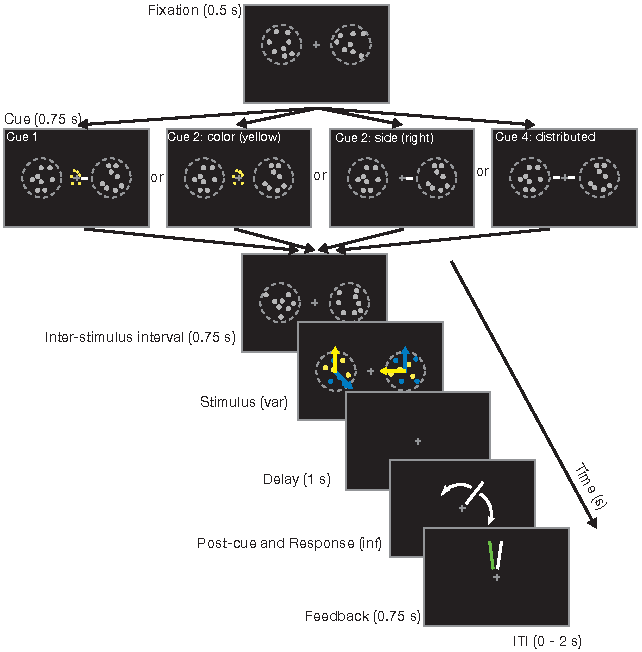
\includegraphics[keepaspectratio,width=0.6\textwidth]{figs_c4/f4_estimationtask.pdf}
\caption[Estimation task]{Estimation task. The task is shown where the cues were side (left or right) and colors (yellow or blue) and observers reported motion direction, but we also ran the reverse where the cues were side (left or right) and motion direction (up or down) and observers reported the color. Observers began each trial by fixating a central cross (Fixation). A pre-cue (Cue) was then shown to indicate to observers which of the four dot patches they should memorize. A brief delay (Inter-stimulus interval) gave observers time to prepare. The dots then became colored and coherent for a variable duration (Stimulus). Finally after another brief delay (Delay) observers were shown a second cue which was used to disambiguate the target stimulus (Post-cue). For example, if the observer was cued to remember the two stimuli on the right, the post-cue might be blue to indicate that of the two stimuli memorized only the motion direction of the blue dot patch on the right should be reported. Observers were given unlimited time to respond (Response) and received feedback before the next trial (Feedback).}
\label{fig:c4f4}
\end{figure}

The estimation task uses the same stimulus as the averaging task, but we now asked observers to recall a single motion direction (rather than the average of two). Observers were cued in different ways to force them to select the stimulus according to different features. To set a baseline for performance we cued observers to the exact target they would later report (Cue 1, Fig. \ref{fig:c4f4}). In the most difficult case (Cue 4: Distributed, Fig. \ref{fig:c4f4}) observers memorized the directions of all four potential targets and were only post-cued after a brief delay about which target should be reported. In the two critical selection conditions observers were asked to memorize either the motion directions of the two patches on the left or right (Cue 2: Side, Fig. \ref{fig:c4f4}) or the two yellow or blue patches (Cue 2: color, Fig. \ref{fig:c4f4}), in the same manner as in the averaging task. In both of these conditions a Post-Cue was used to reveal which of the memorized dot patches had to ultimately be reported. Note that we had observers perform this task in two ways: once selecting by either location (left/right) or color (yellow/blue) and reporting motion direction, as shown in the figure, but also while selecting by either location or motion direction (up/down) and reporting color (see e.g. Fig. \ref{fig:c4f6}). 

\begin{figure}
\centering
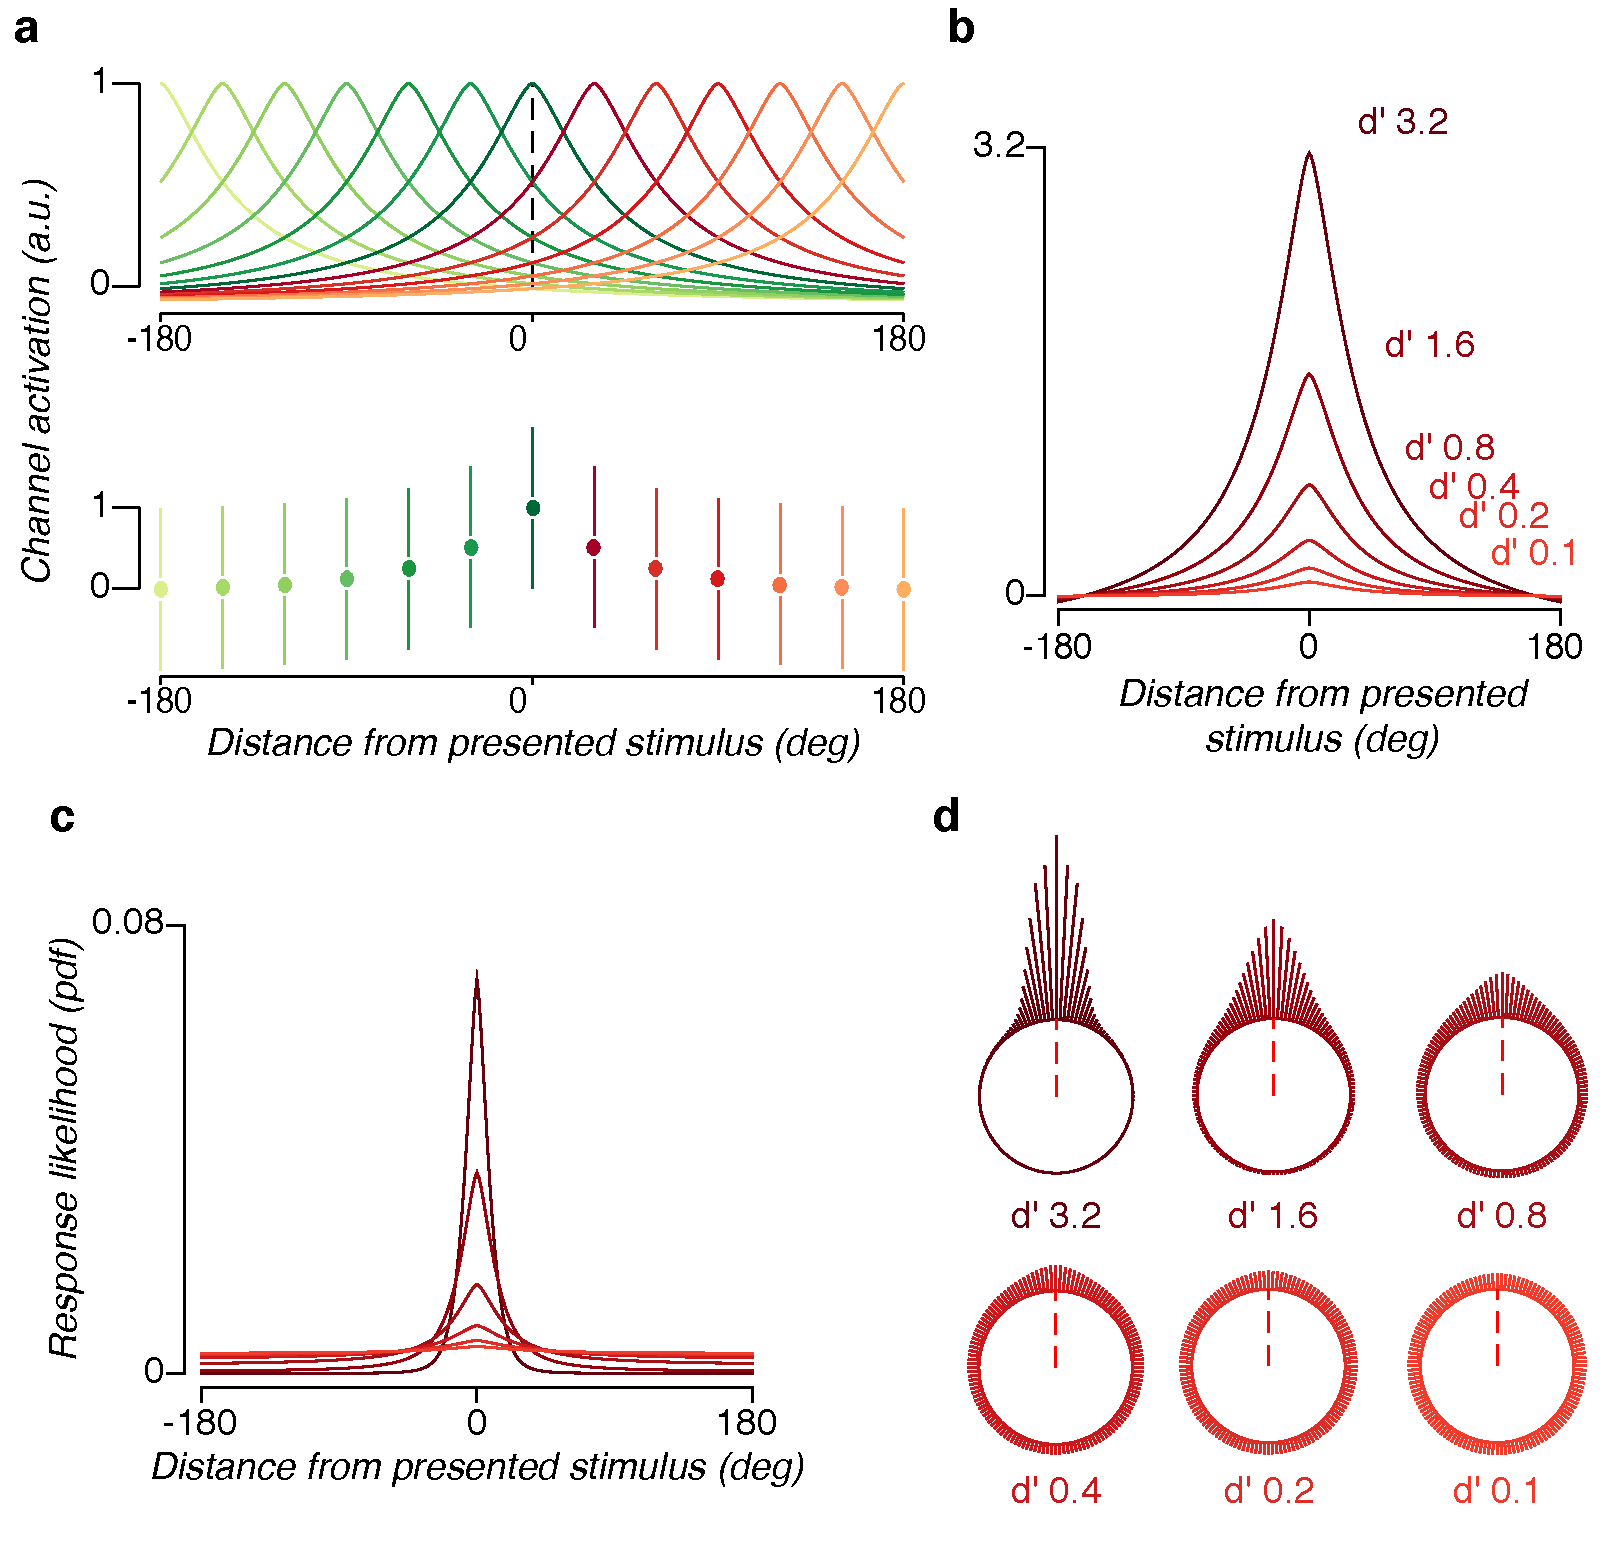
\includegraphics[keepaspectratio,width=0.6\textwidth]{figs_c4/f3_TCC_model.pdf}
\caption[Estimation task model]{Estimation task model. The model of the estimation task is based on an existing model of working memory estimation by \citet{Schurgin2018-vi}. (a) In the model independent channels encode the stimulus with a response profile defined by the psychophysical distance of each channel's preferred response and the stimulus. The channel responses are normally distributed with $\sigma=1$. (b) A free parameter in the model controls the sensitivity of the channels ($d'$), which acts as a multiplicative gain on the amplitudes of each channel response. (c) To read out an estimate of the stimulus angle an observer takes the maximum response over the channels. We show here the full likelihood distribution over all angles, computed numerically (see Methods). (d) The same distributions in (c), the likelihood of response for different values of $d'$, are shown in circular space. (e) To estimate the trial-by-trial likelihood of responses in the estimation task we fit a separate sensitivity parameter for each dot patch, indexed by its relative position to the reported target patch on that trial. The four patches are the reported patch (orange, \textit{target}), the patch on the same side (blue, \textot{side}), the patch on the opposite side with the same feature (pink, \textot{feature}), and the patch on the opposite side with the mismatched feature (green, \textit{distractor}). To decompose bias from sensitivity we weighted the likelihood distributions by $\beta$ weights for each condition. These $\beta$ weights were constrained to sum to 1 (see Methods). Once summed, these define a trial-by-trial likelihood distribution for each observer. Note that for clarity of presentation we are showing the task variant in which colors are reported, while Fig. \ref{fig:C4f4} shows the variant in which motion directions are reported.}
\label{fig:c4f5}
\end{figure}

To understand the data we collected from the estimation task we needed to decompose bias from sensitivity. To do this we employed a simple model of perceptual sensitivity which fits two parameters for each condition (Fig. \ref{fig:c4f5}, see Methods for details). The model encodes the stimulus into a set of independent channels with Gaussian-distributed noise (Fig. \ref{fig:c4f5}a). A single parameter scales the responses of these channels to fit the sensitivity of an observer (Fig. \ref{fig:c4f5}b). To obtain the likelihood of an observer's responses the maximum is taken over the channel responses, resulting in a likelihood distribution (Fig. \ref{fig:c4f5}c). To decompose sensitivity from bias we allowed the channels to separately encode each of the dot patches with a separate sensitivity, then weighted those likelihood functions to create a mixed distribution from which actual trail-by-trial responses would be sampled (Fig. \ref{fig:c4f5}e). We fit all seven parameters of this model (four $\beta$ and three $d'$ parameters) to maximize the likelihood of predicting the responses of each observer. 

\begin{figure}
\centering
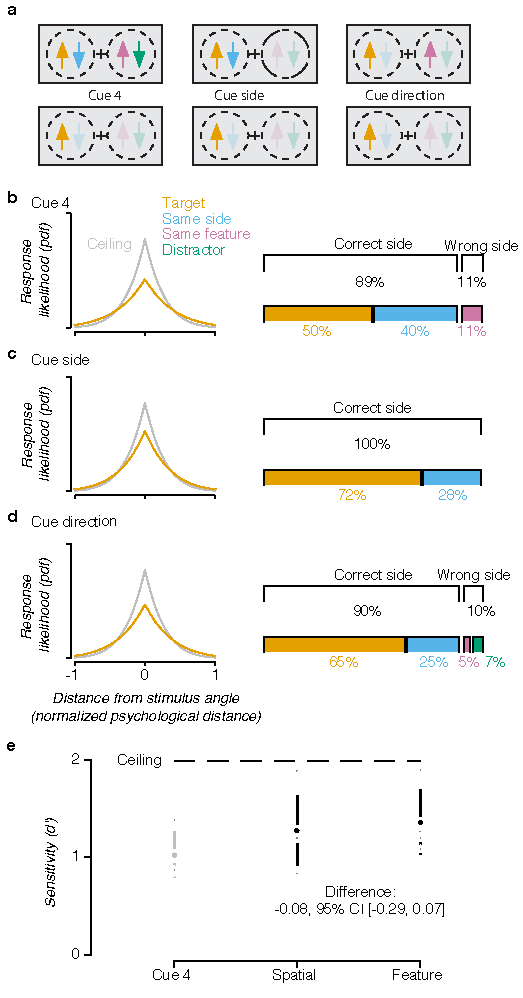
\includegraphics[keepaspectratio,width=0.5\textwidth]{figs_c4/f4b_estimation_perf.pdf}
\caption[Estimation task performance]{Performance in the estimation task. (a) Three of the conditions used in the experiment are shown for trials where selection was performed by the direction of motion and the report was the color. Opacity is used to indicate which dot patches are memorized in each condition and to emphasize that the response in all conditions is identical (reporting the color of a single dot patch). In Cue 4 trials an observer memorized all four colors shown and was then asked to report the color of a single dot patch, e.g. the dots moving upward on the left side (orange arrow, highlighted). In Cue 2 trials the observer either memorized the colors on one side (Cue side) and was post-cued about the direction, or memorized two dot patches moving in the same direction (Cue direction) and was post-cued about the side. (b) The model estimate of sensitivity for each of the four dot patches is shown separated from the probability of reporting about each dot patch. Observers reported about the distractor dot patch less than 2\% of the time. (c-d) Conventions as in (b) for the two cue 2 conditions. (e) Confidence intervals for the \textit{target} dot patch $d'$ parameter are shown for each condition.}
\label{fig:c4f6}
\end{figure}

We compared three conditions in the estimation task, using the Cue 1 condition as a baseline for performance (Fig. \ref{fig:c4f6} and found that all of the variability in performance between conditions was accounted for by the bias parameters. Our main goal was to see whether during the two different forms of selection (Cue side and Cue feature) a difference in sensitivity to the target dot patch emerged. We did not find this to be the case (left panels, orange curves are all identical, Fig. \ref{fig:c4f6}b-d). A direct comparison of these sensitivity parameters between conditions and against the same parameter in the Cue 4 condition showed no differences (Fig. \ref{fig:c4f6}e) between forms of selection, but a substantial advantage to selecting two patches compared to selecting only four. 

While we found no differences in the sensitivity parameters we did find substantial differences in how biased observers were to report about the incorrect dot patches in different conditions (right panels, Fig. \ref{fig:c4f6}b-d). When remembering all four dot patches (Cue 4) we found that observers were only able to report the direction of the correct dot patch half the time. They were nearly equally likely to confuse the patch we asked them to report with the patch on the same side. A small percentage of the time (10.5\%) observers reported about the feature matched stimulus on the wrong side. Performance improved substantially in both conditions where observers were cued to remember just two of the four dot patches. In the Cue side conditions we found that observers were only biased to report about the dot patch on the same side. In the Cue feature conditions we found that observers occasionally reported about all of the irrelevant dot patches with some frequency, indicating a difference in bias due to the form of selection. 

\begin{figure}
\centering
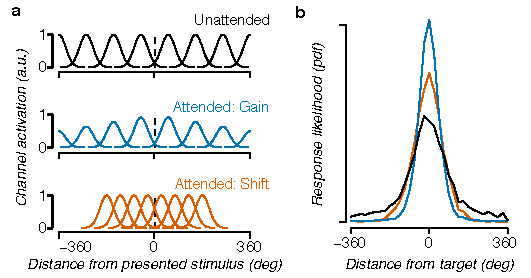
\includegraphics[keepaspectratio,width=0.6\textwidth]{figs_c4/f5_channel_attention.pdf}
\caption[Attention in a channel model]{Implementations of attention in a hypothetical channel model. (a) Examples are shown of how neuron responses might change during attention. (b) Response likelihoods are shown for the different attention models, see Methods for model details.}
\label{fig:c4f7}
\end{figure}

In previous chapters we explored different possible models for how attention could be implemented in sensory representations or their readout. Here again we wanted to explore possible implementations for how neural selection might result in the behavioral changes we observed. An important step toward this goal is to describe a computational linking model which can connect the perceptual measurements described here with measurements of cortical activity. We describe here such a model and demonstrate that it can in theory account for the kinds of shifts in sensitivity and bias that could occur in our task (Fig. \ref{fig:c4f7}).

A plausible linking model has to have channels that are tuned according to functions with thinner response profiles than those described by the psychophysical scaling function (Eq. \ref{eqn:c5psycho}, see also Fig. \ref{fig:c4f5}a). Ultimately the size and number of these channels would need to be constrained by neural data. For our purposes we simply modeled a small number of channels (128) with small variance (circular Von Mises distributions with $\kappa=20$). To simulate read out from such a population during an estimation task we proceeded in two steps. First, we simulated the response to a stimulus by sampling from each channel's response to the stimulus angle, with additive Gaussian noise. Then, to decode the angle stored in the channels we compared the sampled responses to the ideal mean responses for every channel for every possible stimulus angle (Eq. \ref{eqn:c5readout}, i.e. we computed the dot product of the sample vector and the mean channel response vector for each $\theta$). The maximum of this readout step was chosen as the response for that simulated trial. We repeated this 1,000$\times$ and then plotted the distribution of response angles relative to the true stimulus angle (Fig. \ref{fig:c4f7}b).

Changes in sensitivity in such a model can be the result of different manipulations in the channels, such as multiplicative gain or shifts in tuning. Using the simulation we showed that a multiplicative gain or a shift in tuning can both result in changes to the distribution of estimated angles (blue and orange lines, Fig. \ref{fig:c4f7}a and b). Combined with the estimation task we therefore believe that this approach provides a computational linking model to connect measurements of cortical representation to the behavioral measurements. When observers went from memorizing four dot patches to two, whether by location or feature, their perceptual sensitivity improved substantially (Fig. \ref{fig:c4f6}e). We expect that enhancement to be the result of both changes in sensory representation but also potentially changes in the readout (see Chapter 3). Combining this computational linking model with measurements of cortical activity will make it possible to evaluate whether the scale of observed changes in cortical representation are sufficient to account for the behavioral effects of selective visual selection. 

\section{Discussion}

Using perceptual averaging and estimation we have demonstrated that selection by spatial location and by feature both enhance perceptual sensitivity by a similar amount. We observed small differences in task performance which were well accounted for by bias. This showed that selection changes how likely observers were to report about the wrong dot patch, but did not change the strength of their encoding of the dot patches. These results make a compelling case for the hypothesis that selective visual attention has a shared neural implementation across different visual features. Our results also confirm that selection by spatial location may occur prior to selection by other features, paralleling our knowledge of the physiological structure of early visual cortex. 

Many early experiments that compared different forms of visual selection came to the conclusion that spatial location is primary in some way \citep{Liu2007-ed,Treisman1980-gu,Tsal1988-qx,Snyder1972-og,Hillyard1984-qk,Harter1982-vj,Soto2004-cs}. In general, this idea that spatial selection precedes feature-based selection matches cortical physiology. Early visual cortex is organized retinotopically \citep{Wandell2007-pr} and the earliest visual areas are sensitive to specific visual features at particular retinotopic locations \citep{Kuffler1953-qw,Hubel1959-fo,Hubel1962-pn}. The progression from local simple features to more global complex features provides one explanation for the pattern of bias which we observed. We found that when selecting by spatial location observers were able to easily ignore the dot patches in the other visual field, consistent with an implementation preventing those dot patches from being fully processed. But to select dot patches by feature observers were required to not select by location, perhaps allowing processing to continue on those irrelevant dot patches. This possibility might explain why observers were sometimes biased to the feature mis-matched dot patches on the same and opposite side even when selecting by feature. Despite this bias, observers were nevertheless equally sensitive, i.e. their responses were just as variable, when selecting by location or by feature.